% 
% Annual Cognitive Science Conference
% Sample LaTeX Paper -- Proceedings Format
% 

% Original : Ashwin Ram (ashwin@cc.gatech.edu)       04/01/1994
% Modified : Johanna Moore (jmoore@cs.pitt.edu)      03/17/1995
% Modified : David Noelle (noelle@ucsd.edu)          03/15/1996
% Modified : Pat Langley (langley@cs.stanford.edu)   01/26/1997
% Latex2e corrections by Ramin Charles Nakisa        01/28/1997 
% Modified : Tina Eliassi-Rad (eliassi@cs.wisc.edu)  01/31/1998
% Modified : Trisha Yannuzzi (trisha@ircs.upenn.edu) 12/28/1999 (in process)
% Modified : Mary Ellen Foster (M.E.Foster@ed.ac.uk) 12/11/2000
% Modified : Ken Forbus                              01/23/2004
% Modified : Eli M. Silk (esilk@pitt.edu)            05/24/2005
% Modified : Niels Taatgen (taatgen@cmu.edu)         10/24/2006
% Modified : David Noelle (dnoelle@ucmerced.edu)     11/19/2014
% Modified : Roger Levy (rplevy@mit.edu)     12/31/2018


%% Change "letterpaper" in the following line to "a4paper" if you must.

\documentclass[10pt,letterpaper]{article}

\usepackage{cogsci}
\usepackage{color}
\usepackage{tikz}
\usetikzlibrary{bayesnet}
\usepackage{amsmath,amssymb,amsfonts,amsthm}
\usepackage{pgfplotstable}
\usepackage{csvsimple}
\usepackage{booktabs}
\cogscifinalcopy % Uncomment this line for the final submission 

\usepackage{pslatex}
\usepackage{apacite}
\usepackage{float} % Roger Levy added this and changed figure/table
                   % placement to [H] for conformity to Word template,
                   % though floating tables and figures to top is
                   % still generally recommended!

%\usepackage[none]{hyphenat} % Sometimes it can be useful to turn off
%hyphenation for purposes such as spell checking of the resulting
%PDF.  Uncomment this block to turn off hyphenation.


%\setlength\titlebox{4.5cm}
% You can expand the titlebox if you need extra space
% to show all the authors. Please do not make the titlebox
% smaller than 4.5cm (the original size).
%%If you do, we reserve the right to require you to change it back in
%%the camera-ready version, which could interfere with the timely
%%appearance of your paper in the Proceedings.

\definecolor{Red}{RGB}{255,0,0}
\definecolor{Green}{RGB}{10,200,100}
\definecolor{Blue}{RGB}{10,100,200}
\definecolor{Orange}{RGB}{255,153,0}

\newcommand{\denote}[1]{\mbox{ $[\![ #1 ]\!]$}}
\newcommand*\diff{\mathop{}\!\mathrm{d}}
\newcommand{\red}[1]{\textcolor{Red}{#1}}  
\newcommand{\soph}[1]{\textcolor{Green}{[sb: #1]}}  
\newcommand{\mht}[1]{\textcolor{Blue}{[mht: #1]}}  

\title{How many observations is one generic worth?}
 
%\author{{\large \bf Michael Henry Tessler$^{1}$ (tessler@mit.edu)}, {\large \bf Sophie Bridgers$^{2}$ (sbridge@stanford.edu)}, and {\large \bf Joshua B. Tenenbaum$^{1}$ (jbt@mit.edu)} \ \\
%  $^{1}$Department of Brain and Cognitive Sciences, MIT \\
%   $^{2}$Department of Psychology, Stanford University}
   
  \author{{\large \bf Michael Henry Tessler (tessler@mit.edu)} \\
  Department of Brain and Cognitive Sciences, MIT
  \AND {\large \bf Sophie Bridgers (sbridge@stanford.edu)} \\
  Department of Psychology,  Stanford University
    \AND {\large \bf  Joshua B. Tenenbaum (jbt@mit.edu)} \\
  Department of Brain and Cognitive Sciences, MIT
  } 
   
   


\begin{document}

\maketitle


\begin{abstract}
% From CDS, but too long here - need to get it down to 150 words: 
%Generic language (e.g., ``Birds fly'') conveys generalizations about categories and is a simple and ubiquitous way of learning beyond direct experience. The meaning, and hence the belief-updating capacity, of generic language is hard to specify however (e.g., penguins don't fly), owing to extreme forms of content and context-sensitivity. Tessler \& Goodman (2019) proposed that generics are a kind of vague quantifier (a la ``some'', ``most'') which operate over richly structured prior knowledge. Their computational model is mathematically equivalent to simple Bayesian belief-updating based on a single positive example. This rather surprising mathematical connection between learning from generic language and learning from observations suggests a developmental mechanism for meaning acquisition, namely: semantics can co-opt more basic mechanisms of belief-updating from observations. Relatedly, Csibra \& Shamsudheen (2015) argue that generics are an inherently non-verbal but pedagogical phenomenon, which can be understood by pre-linguistic infants via intentional reference to a member of a kind. In a quantitative study with adults, using a diverse set of stimuli covering a range of prior beliefs, we compare the belief-updating capacity of generic language to that of single observations, both presented pedagogically and incidentally. We find that generics convey stronger generalizations than single observations even when presented pedagogically, which we operationalize in two distinct ways. This work raises new questions about the contextual parameters that would support learning generic-like generalizations from pedagogical demonstrations in infancy and early childhood.

% 150 word shortening
Generic language (e.g., ``Birds fly'') conveys generalizations about categories and is essential for learning beyond our direct experience. The meaning of generic language is notoriously hard to specify, however (e.g., penguins don't fly). \citeA{tessler2019language} proposed that generics are a kind of vague quantifier (a la ``some'', ``most'') operating over structured prior knowledge. We show how their model is mathematically equivalent to Bayesian belief-updating based on a single positive example, suggesting a deep connection between learning from experience and learning from language. Relatedly, \citeA{csibra2015nonverbal} argue that generics are inherently pedagogical, understood by infants as referring to a member of a kind. In a quantitative study with adults, we compare the belief-updating capacity of generic language vs. observations, which vary in both the number of observations and whether they are presented pedagogically or incidentally. Generics convey stronger generalizations than even single pedagogical observations, raising new questions about how these generalizations are learned in infancy and early childhood.


\textbf{Keywords:} 
generic language; Bayesian learning; belief updating; pedagogical sampling; observational learning
\end{abstract}


\section{Introduction}

The world is a confusing and confounding place, but forming the right kind of generalizations eases our navigation of the environment. A critical source of information for acquiring generalizable knowledge is other people in the world. There are two major routes for acquiring such knowledge from others: observing their actions and listening to the words they say. 
%Two critical routes for acquiring generalizable knowledge is by directly observing the world ourselves, including others' actions, or by learning from others via language. %I eased this dichotomy because there are other routes to learning such as intervention and exploration; and we also observe other people...not sure if we need to get into this but something to keep in mind -- i.e., observing the world often involves ob
Indeed, one hallmark of human intelligence, present in infancy and childhood, is our capacity to draw strong generalizations from just a few examples~\cite<e.g.,>{gopnik2001causal, gopnik2004theory, gweon2010infants, gweon201116, tenenbaum2006theory}. At the same time, abstract generalizations can also be conveyed with language, using what is called \emph{generic language} \cite<or, \emph{generics}; e.g., ``Swans are white'';>{carlson1977reference, leslie2007generics,Gelman2002,tessler2019language}.
Given that generalizations can be acquired from observation and from language, then there must be some relationship between the two. There must be some point at which the strength of an inductive generalization drawn from experience is equal to that of a generalization learned from language  (Figure \ref{fig:cartoon}).
%how many observations is one generic worth?
%What is the relationship between learning from language and learning from experience?
%When is 
%between inductive generalizations drawn from observations (either those presented pedagogically vs. not) and those learned from generics? \soph{This question is hard to parse. Not sure what it means...}

Not all observations of others' actions are created equal.
Watching an informed and cooperative interlocutor intentionally convey an example via a demonstration is a stronger signal than if the observation is observed by happenstance \cite{shafto2012learning}, which can result in more robust generalizations in adults and children \cite{goodman2009cause, butler2012preschoolers}. % \red{(cite butler and markman)}.
Thus, a crucial question is not only how many observations is one generic worth but what kind of observations are they -- socially demonstrated or just incidentally observed?

\begin{figure}[t]
\begin{center}
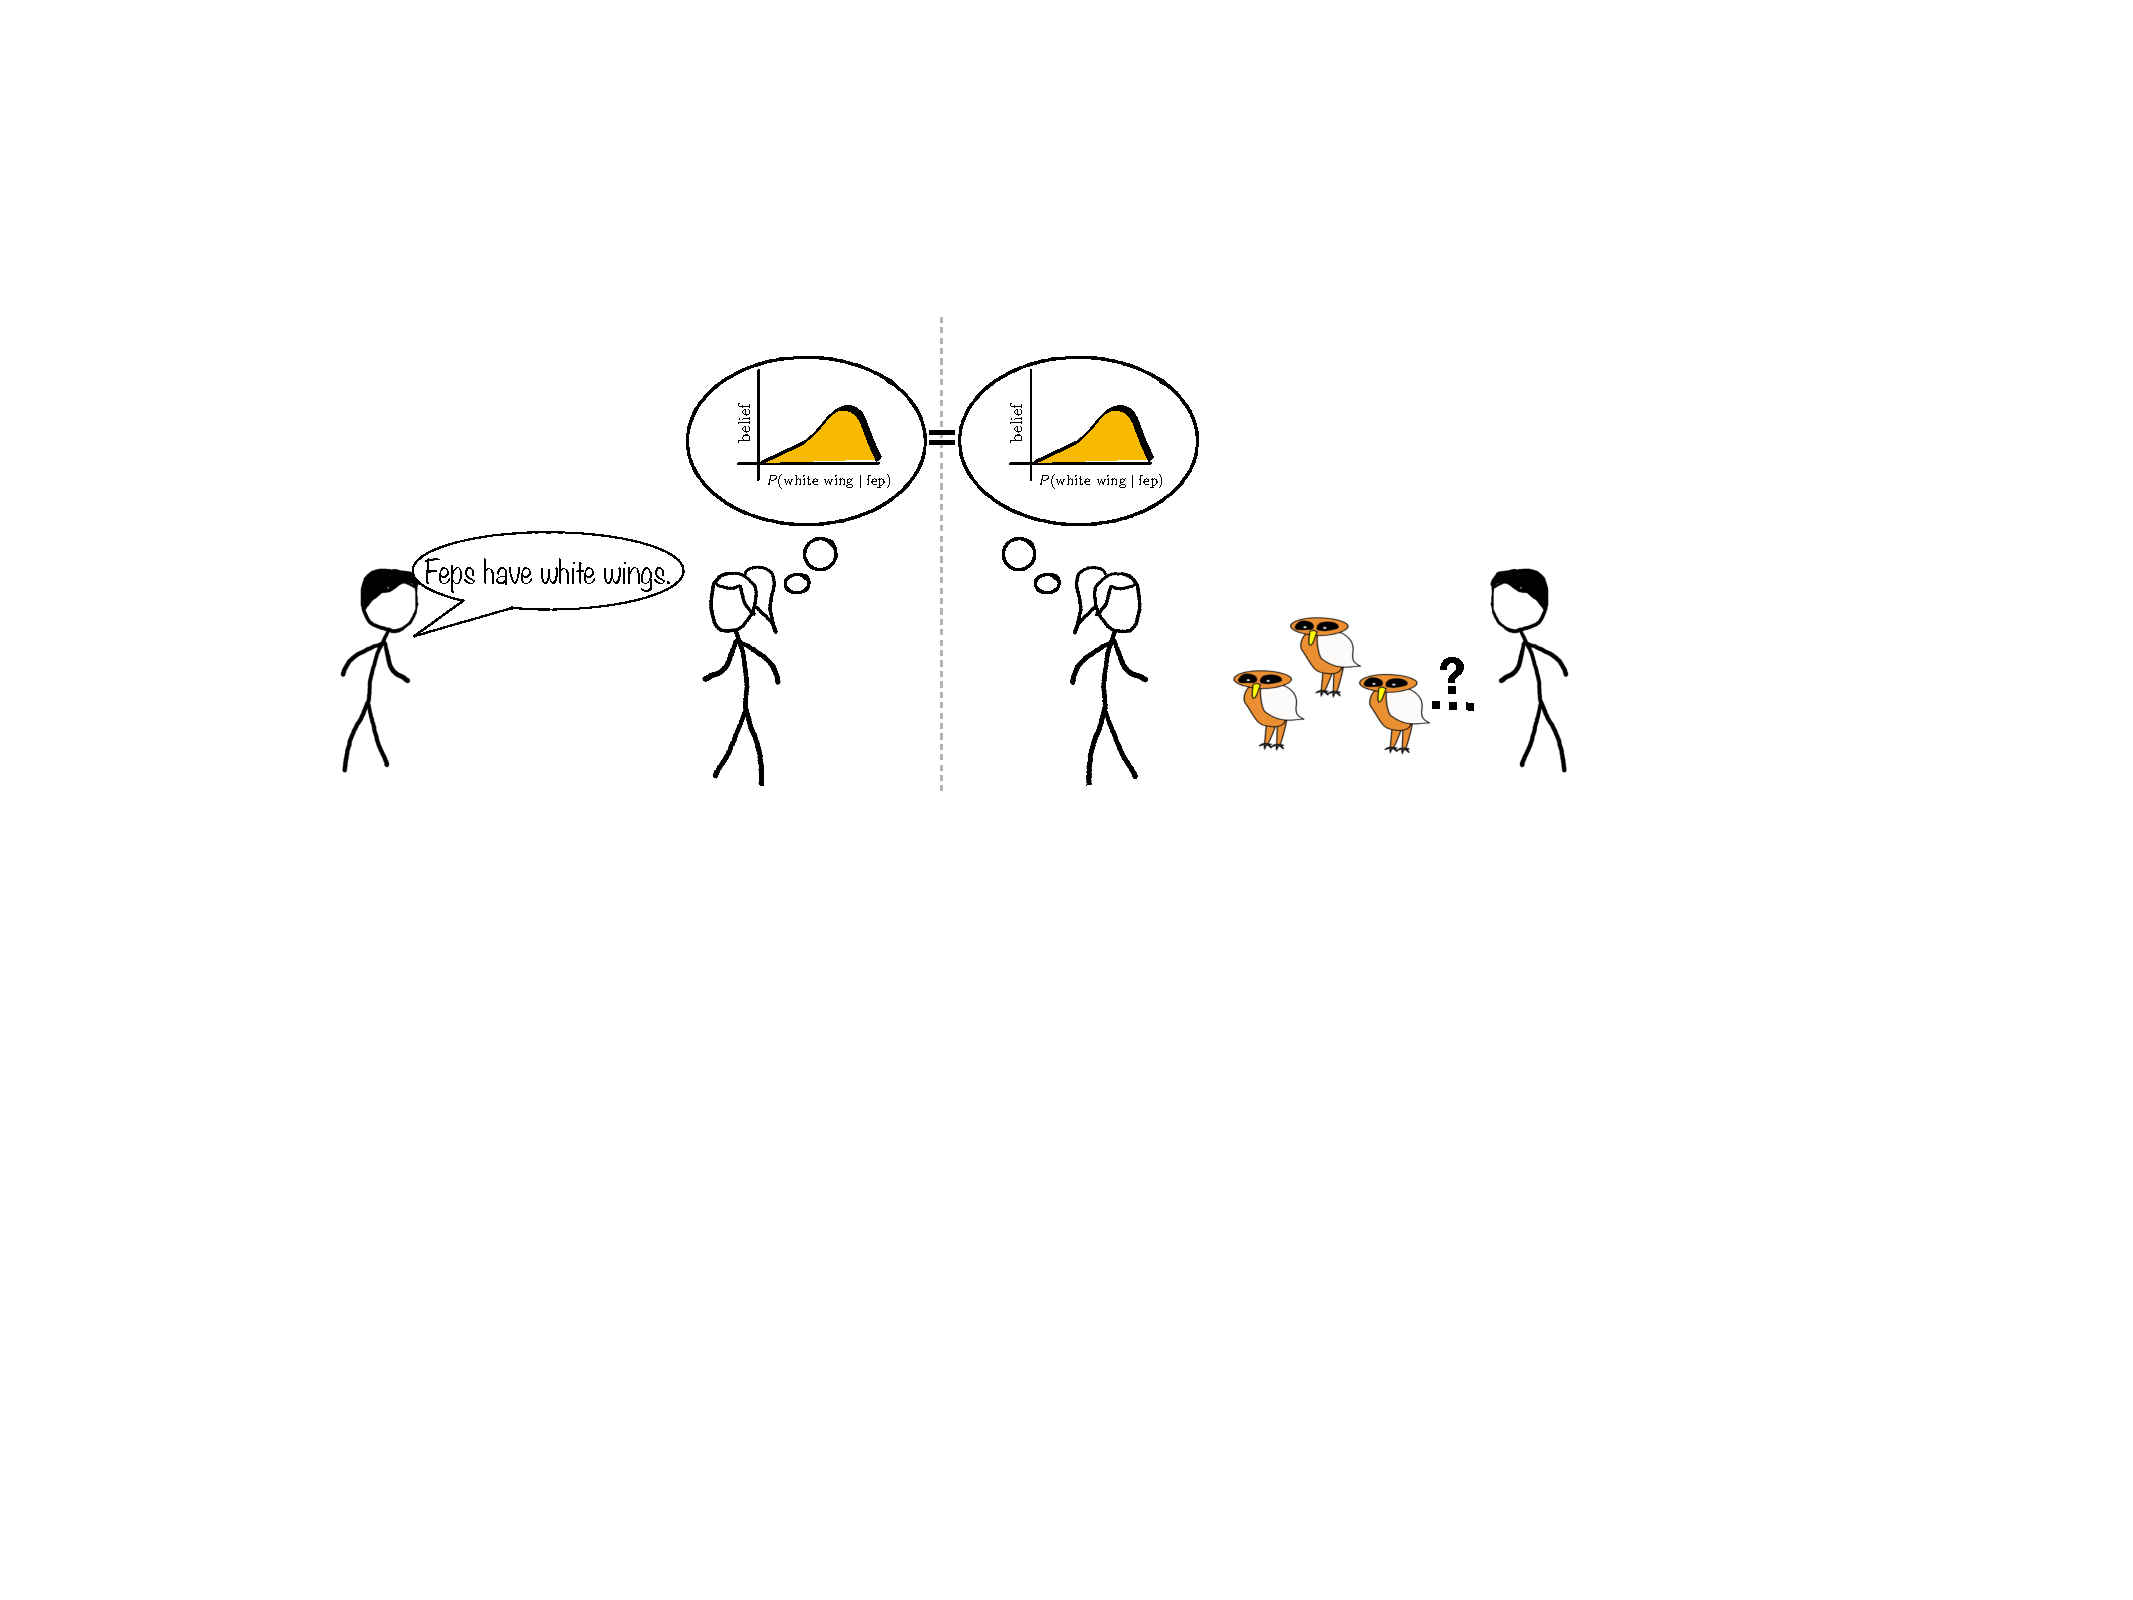
\includegraphics[width=\linewidth]{figs/cartoon-fig.pdf}
\end{center}
\caption{Generalizations about categories -- expressed via degrees of belief of an instance of the category having the feature -- are learned both from generic language (left) and direct observations (right). When is the strength of generalization drawn from examples equal to that drawn from a generic statement? Or, how many observations is one generic worth?}
\label{fig:cartoon}
\end{figure}

%We understand the lightning tends to strike tall objects and that smoking causes cancer, but how do we come to know these generalizations?

Articulating the precise relationship between learning from examples and learning from language is difficult because learning from linguistic utterances operates via the \emph{truth conditions} of the utterance, which are more often than not difficult to specify precisely. %because the meanings can change dramatically depending on the context.
Generics are a clear case of context-specific language:  while \emph{Triangles have three sides} should be taken to mean that exactly 100\% of triangles have three sides, \emph{Swans are white} is more tolerating of exceptions (i.e., there are black swans); \emph{Mosquitoes carry malaria} is an example of a generic that conveys a very weak generalization: the vast majority of real-world mosquitoes do not carry the virus. 
To capture this heterogeneity, \citeA{tessler2019language} proposed a meaning for generics that is similar to that of quantifiers (e.g., \emph{some}, \emph{most}, or \emph{all}) but which has an uncertain truth-conditional threshold; that is, the \emph{quantificational strength} is underspecified by the utterance but is determined in context through Bayesian reasoning. 
This model of generics as a kind of vague quantifier bears an intriguing relationship to models of belief-updating from observations: With some minimal assumptions, a generic updates beliefs in a way analogous to a single, pedagogically-presented example \cite{tessler2020learning}. 
%\mht{decide whether to keep this citation to the ms, or just present here as if for the first time...?}



The relationship between the meaning of generics and pedagogical examples has independently been interrogated and elucidated to understand infant cognition \cite{csibra2015nonverbal}.
\citeA{csibra2015nonverbal} argue that pedagogical reference to an instance of a kind (e.g., using ostensive cues such as pointing) can be interpreted by pre-verbal infants as a symbolic reference to the entire kind or class.  
%because infants conceive of objects as \emph{instances of kinds},% \cite{prasada2019instance}, 
Then, any demonstration that may occur during this pedagogical episode can be understood by the infant as predicating the demonstrated property of the kind (e.g., if an object is demonstrated to squeak, infants not only learn that the specific, demonstrated exemplar squeaks but infer that this category of objects squeaks).
The authors argue that this act is a non-verbal analogue of a generic statement.

Thus, proposals from two rather different theoretical frameworks---Bayesian models of semantics and infant cognitive development---point to the rather intriguing hypothesis that the information content of a generic might be equivalent to that of a single, pedagogically-presented example.
On the other hand, generics are often commonly expressed with plurals in many languages including English (e.g., \emph{Dogs bark}), and a plural should be a cue that the literal meaning goes beyond a single example.
Furthermore, the relationship between generics and pedagogical examples that \citeA{csibra2015nonverbal} propose for preverbal infants may not be the same throughout development; indeed, 3- and 4-year-olds can interpret the ostensive cue of pointing as a signal that the information conveyed is not generalizable, but rather specific to the exemplars referenced by the point \cite{meyer2013pointing}.
%Furthermore, the prediction from the vague quantifier model of generics is contingent on the assumption that prior beliefs about the quantificational strength of a generic (i.e., what kind of generalization does a generic convey?) is uniform (i.e., all quantificational strengths are equally likely \emph{a priori}); those prior beliefs may turn out to not be uniform but skewed towards higher thresholds (e.g., a generic, in the abstract, is more likely to imply \emph{most} than imply \emph{some}), then it would be worth a larger number of examples. 
%\soph{I like this discussion! I think the point about the model may need to be spelled out a bit more for non-computational readers.}

%There are two suggestions for how learning from examples might relate to learning from generics.
%The first is derived via the comptuational model of \cite{Tessler2019psychrev}: We show how the vague quantifier model relates to Bayesian belief-updating from observations. 
%Under the most minimal of assumptions, the literal listener component of   \cite{Tessler2019psychrev}reduces to belief-updating given a \emph{single, positive example} and the pragmatic listener model introduced by  \cite{Tessler2020genint} would amount to a belief-updating model given a pedagogically presented single example.

In this paper, we take an empirical approach to investigate the relationship between learning from examples and learning from generic language by attempting to quantify the \emph{exchange rate} between generics and observations. 
We first describe the theoretical proposals in more detail before the experiments. 
Contra the theoretical proposals, we find that in adults, a generic is worth about three or four pedagogically sampled examples. 
We discuss the implications of this relationship, as well as its potential context-sensitivity and development.
%\soph{The notion of examples v. non-social observations is a bit muddled. The introduction seems to start out contrasting observations of the world and learning from others; but here all examples are presented by people, it's just whether they are accidental or pedagogical. I think we may want to draw that distinction out earlier and also include some information about accidental v. pedagogical.} 
%\mht{i put a stub for a paragraph after para1 for discussing pedagogy (and potentially, vs. accident)}



\section{Theoretical Motivation}
%\soph{this section felt a bit redundant with the introduction. I'm not sure we need it. We could merge with information above.}

We highlight two proposals in the literature concerning the precise relationship of learning from observations and learning from generics.  The first is a computational modeling approach to generic language \cite{tessler2019language}. The second is derived from a view of infants' understanding of objects and kinds \cite{csibra2015nonverbal}. 

\subsection{Generics as vague quantifiers}

Generic statements are difficult to formalize because what they mean in terms of \emph{property prevalence} (e.g., how many instances of the category have the property) can change dramatically depending on the statement.
Generics can be felicitously uttered about features with variable levels of prevalence (e.g., ``Dogs have four legs.''~[99\%]~vs.~``Mosquitoes carry malaria.''~[$<1\%$]), and the truth of two generics about properties with the same prevalence can be judged differently (e.g., ``Robins lay eggs'' is true~vs.~``Robins are female'' is false or at least odd, even though in both case roughly 50\% of robins have the feature). 
This heterogeneity has lead many theorists \cite<e.g.,>{leslie2007generics} to discard the standard, truth-functional tools from semantics.
\citeA{tessler2019language} took a different approach: They proposed treating a generic as a kind of vague quantifier by coupling the standard tools of semantics with probabilistic models of cognition. 

The truth conditions of quantifiers can be formalized as threshold functions on the property prevalence $x$ (e.g., $\denote{some} = x > 0$; $\emph{most}= x > 0.5$; $\denote{all} = x = 1$). \citeA{tessler2019language}'s model for a generic is similar in its truth conditions---$\denote{\emph{gen}} = x > \theta$---but treats the semantic threshold variable for the generic as underspecified. 
Formally, their model puts a probability distribution over the threshold variable---$\theta \sim P(\theta)$---following a similar formal treatment of vague adjectives like \emph{tall} \cite{lassiter2017adjectival}. 
The underspecified threshold combines with a listener's prior knowledge about categories and properties $P_f(x)$ to yield the following model of generic interpretation.
\begin{align}
P (x, \theta \mid \denote{gen}) = P (x, \theta \mid x >  \theta) &\propto \delta_{x > \theta} \cdot P(\theta) \cdot P_f(x)  \label{eq:L0}
%P(x, \theta \mid gen) \propto P(x) P(\theta) \delta_{\denote{gen}= x > \theta}
\end{align}
The prior distribution $P_f(x)$ is a distribution over the prevalence of feature $f$ (which can be relativized to a set of alternative categories). This distribution is an object of theoretical interest in its own right, which has been investigated extensively in the original presentation of this model \cite{tessler2019language,tessler2020learning}. 

The literal contribution of the generic statement is a threshold on prevalence, which takes the form of a Kronecker delta function $\delta_{x > \theta}$ that returns the value of 1 when the literal meaning is true ($x > \theta$) and 0 when it is false. 
Of particular interest for our purposes is a mathematical relationship pointed out in \citeA{tessler2020learning}, which occurs when we compute the marginal posterior distribution on prevalence $P(x \mid \denote{gen})$ by integrating over the listener's uncertainty about the threshold variable. 

\begin{align}
P(x \mid \denote{gen}) &=  \int_{0}^{1} P (x, \theta \mid \denote{gen}) \mathop{}\!\mathrm{d}\theta \nonumber
\\
& \propto  \int_{0}^{1} \delta_{x > \theta}  \cdot P_f(x) \cdot 1 \mathop{}\!\mathrm{d}\theta \nonumber  = \int_{0}^{x} P_f(x) \mathop{}\!\mathrm{d}\theta + \int_{x}^{1} 0 \mathop{}\!\mathrm{d}\theta \nonumber  \\
 &    = P_f(x) \int_{0}^{x} \mathop{}\!\mathrm{d}\theta   =  P_f(x) \cdot x  = P_f(x) \cdot P(\texttt{H} \mid x; n=1)\label{eq:L0d}
\end{align}

Since $P(\theta)$ is a uniform probability distribution, it can be replaced with a constant $1$. On the second line, we separate the integral into two regions, corresponding to whether the utterance is true (left-term) or false (right term).
Since $P_f(x)$ does not depend upon theta, it can be moved outside of the integral, which then results in the formula on the third line. 
What is noteworthy is that the vague quantifier model of generics is equivalent to a model of belief-updating from observations: $P(\texttt{T} \mid x; n=1)$ represents the probability of observing a single positive outcome ($\texttt{T}$, e.g., a coin landing on heads) from a single example (one coin flip; $n=1$). 

Critically, this hypothesis that a generic is worth (in inductive strength) the same as a single positive observation is a hypothesis about the \emph{literal} meaning of a generic, without taking into account pragmatic interpretations \cite{grice1975logic}. % only manifested at the level of a literal listener.
\citeA{tessler2020learning} argue that generic interpretation should be understood not via its literal interpretation but as a pragmatic interpretation (see also \citeNP{vanrooij2019generics} for a similar argument). 
If this is the case, we would expect a generic to be equivalent to a single, pragmatically-enriched (or, pedagogically understood) example. 

%This number of observations depends upon the prior distribution over the semantic threshold $P(\theta)$, which \citeA{tessler2019language} assumed to be uniform $\theta \sim Uniform(0,1)$ (in the first line of the derivation, we replaced $P(\theta)$ with $1$).

%With a different prior distribution on thresholds, one would derive a different relationship between generics and observations.

%Additionally,
\subsection{Non-verbal generics}

A second proposal for the relationship between belief updating from generic language and belief updating from observations comes from \citeA{csibra2015nonverbal}. 
They argue that  when preverbal infants observe an instance of a novel category (call it a \emph{blicket}), they not only have the capacity to individuate this object as a singular entity (i.e., \emph{this is a blicket}) but also have the capacity to see the object as an index to the kind (i.e., this blicket is a pointer to the kind \textsc{blickets}). 
Because of infants' sensitivity to ostensive cues \cite<i.e., natural pedagogy;>{csibra2009natural}, when an object is presented to an infant with pedagogical cues, the infant can interpret the object, not as a singular entity, but as an index to the kind; then, if a property is predicated of that object (e.g., the blicket is shown to squeak), it will be taken by the infant to apply to the kind as a sort of non-verbal generic: \emph{Blickets squeak}.\footnote{Of course, the pedagogical context must signal an event wherein the teacher is aiming to inform the learner about the category and not, say, about a special member of the category. We return to this point in the Discussion.} This view also draws a direct connection between generics and a single, pedagogical example. \footnote{It should be noted that the account of \citeA{csibra2015nonverbal} is intended to be applied to infant cognition. There is no direct or indirect link proposed for this view to be applied to adult cognition or even the cognition of young children who have acquired their first language. In fact, there may be empirical bases to believe this account would not apply to cognition broadly.
%(Baldwin ...).} 
Thus, this argument should be understood as an application of the account of \citeA{csibra2015nonverbal} and not a direct theoretic consequence of it.} 

\section{Experiments}


We develop an empirical paradigm where participants learn about a novel category from examples, from generic language, or both. Participants are then asked to judge the likelihood that a future instance of a category would have the property \cite<cf.,>{Gelman2002,Cimpian2010a,tessler2020learning}.
We titrate the number of examples participants observe in order to determine the point at which the strength of the generalization implied by examples is equal to that of a generic statement (i.e., the \emph{exchange rate} between generics and observations). 


\begin{figure}[t]
\begin{center}
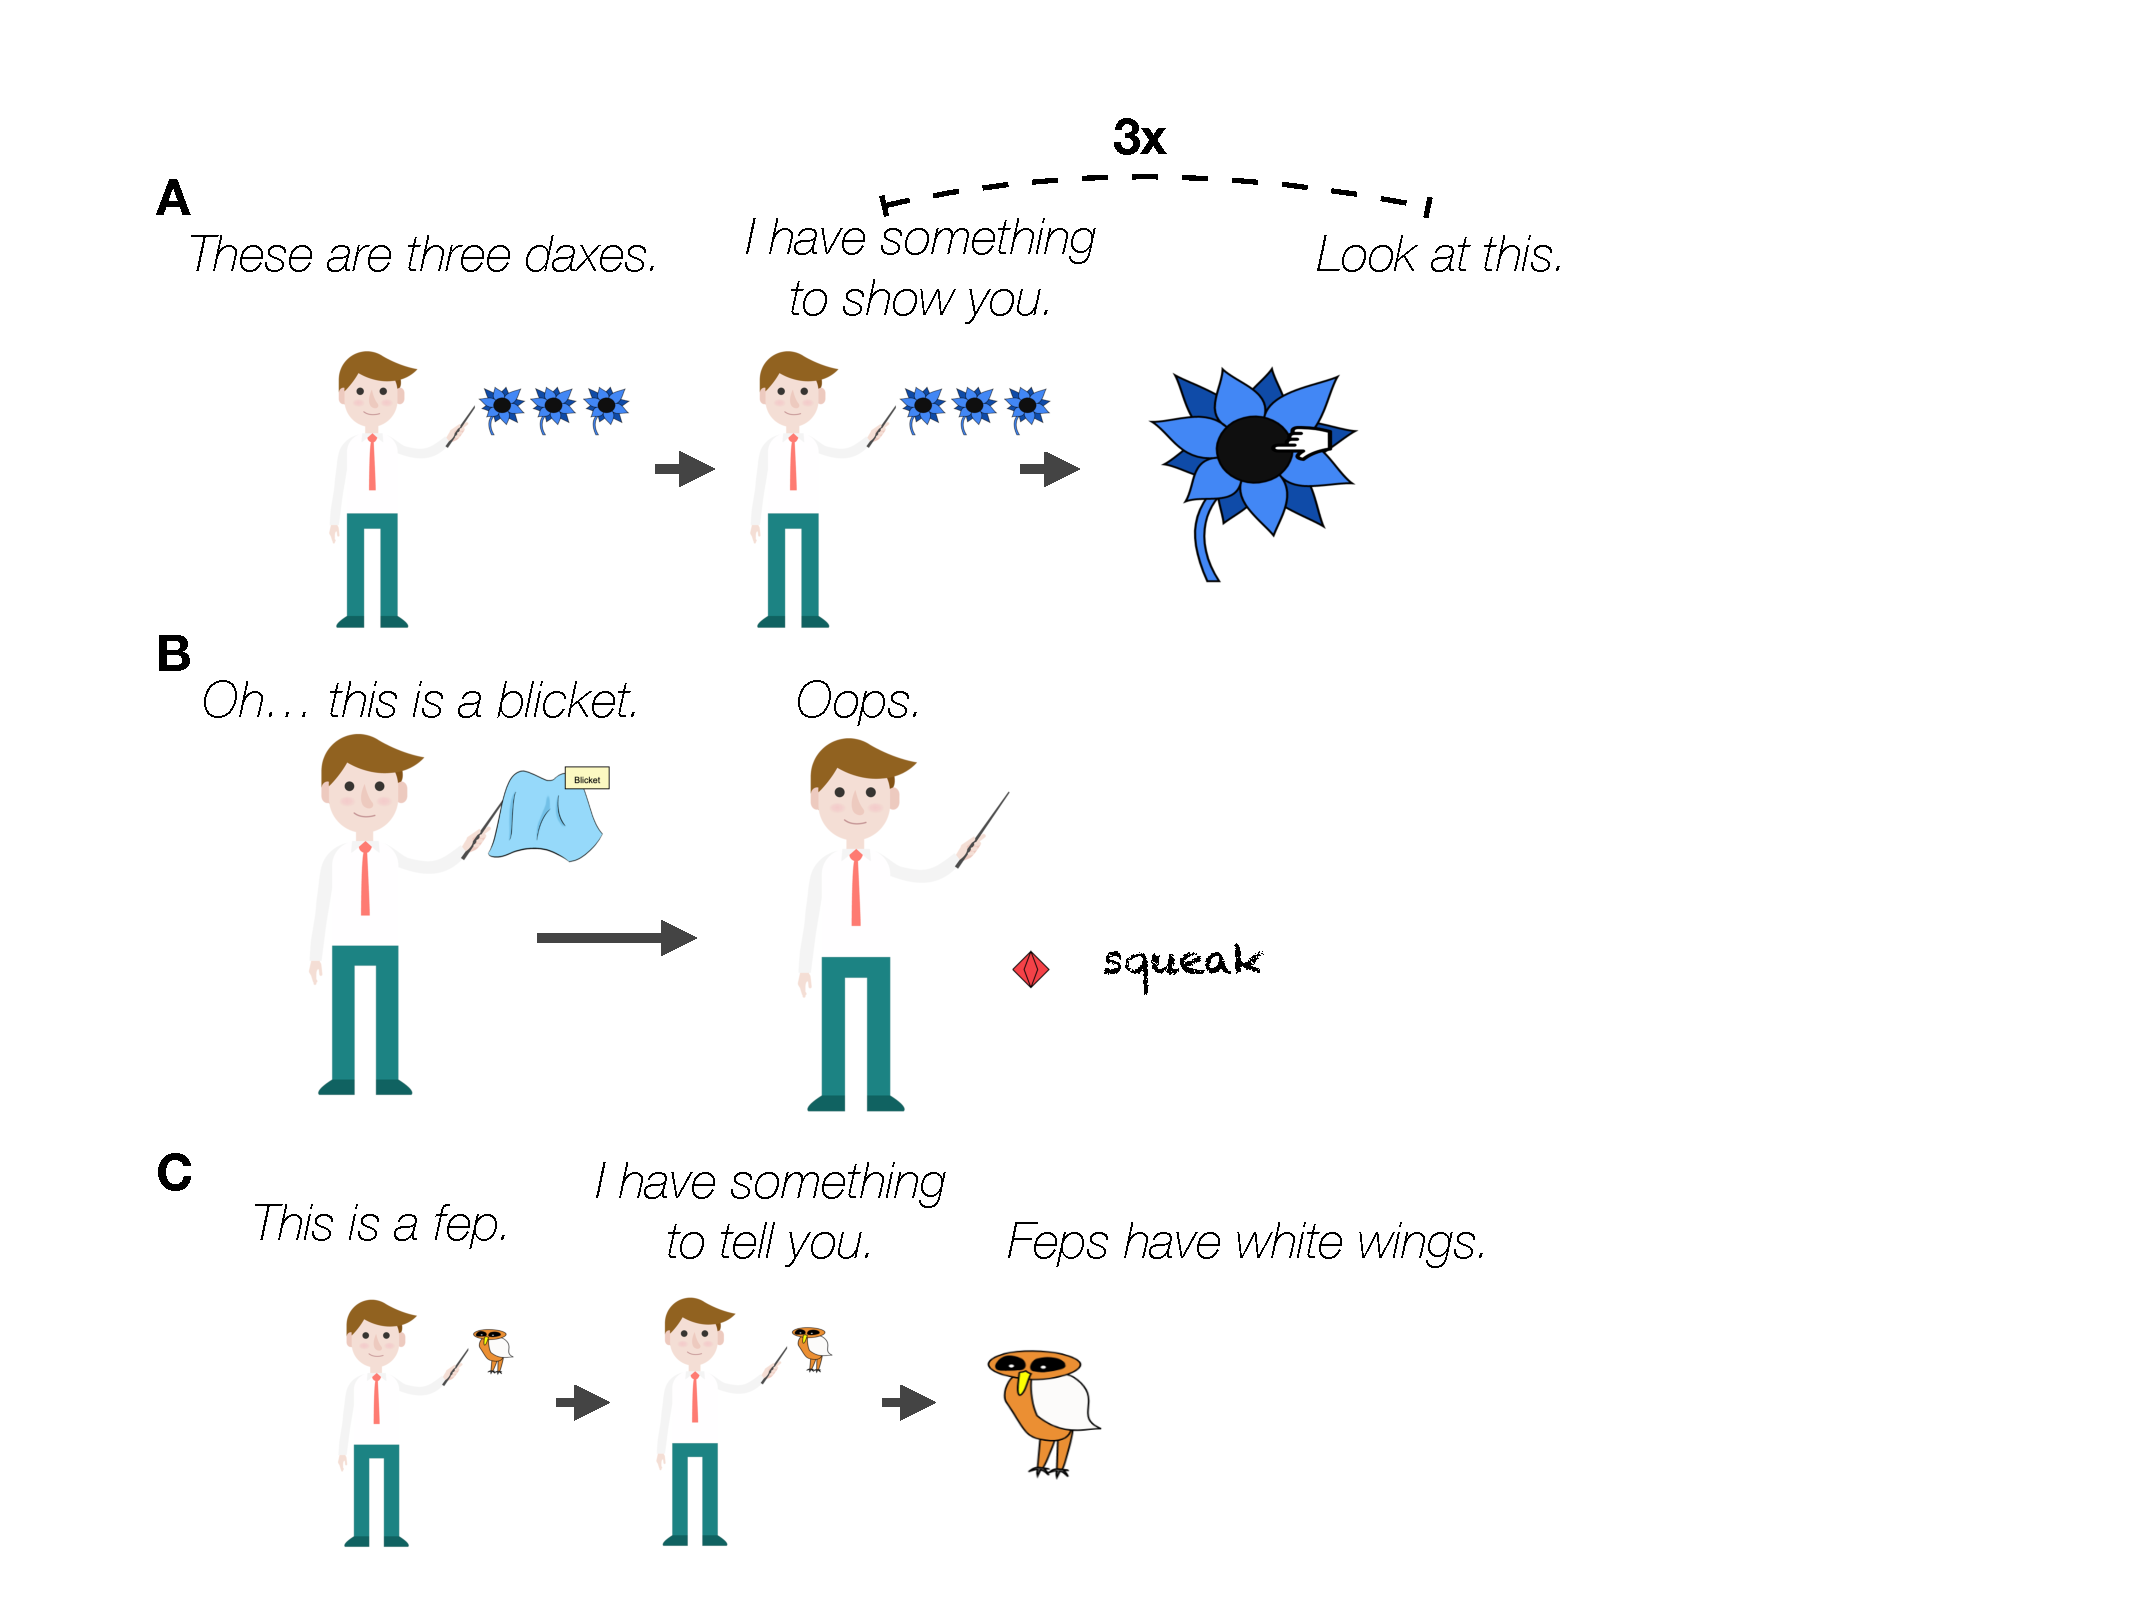
\includegraphics[width=\linewidth]{figs/expt-cartoon.pdf}
\end{center}
\caption{Overview of three conditions of the experiment. Each condition shows a different item that was used. A: 3x Pedagogical Example. The demonstration of the feature repeats 3 times. B: 1x Accidental Example. The speaker is seemingly learning about the object in the experiment (the object appears labeled, but hidden underneath a cloth). C: Generic + Pedagogical Example. Generic statement along with an intentionally demonstrated example.}
\label{fig:expt}
\end{figure}


\subsection{Experiment 1}

%\subsubsection{Method}

\noindent\textbf{Participants}
We recruited 465 adult participants from Amazon's Mechanical Turk. 
By experimenter error, 38 participants were able to do the experiment multiple times (comprising a total of 106 submissions); we only used each participant's first submission, leaving 397 submissions from unique participants. 
Participants were restricted to those with U.S. IP addresses with at least a 95\% work approval rating. 
In addition, participants were required to pass a simple language comprehension test that we deployed in order to weed out bots and other bad-faith participants. 
%The test involved a sentence in which a named speaker (e.g., Joseph) says to a named listener (e.g., Elizabeth) ``It's a beautiful day, isn't it?''. 
%Participants were asked to type in a text box to whom the speaker (in this case: Joseph) is talking (i.e., Elizabeth).
%Speaker and listener names were randomized in a way that could not be read off the source .html file.
%Participants were given three attempts to correctly identify the listener. 
%If they did not succeed within 3 attempts, they would be unable to proceed with the experiment.
Since participants who fail this check are required to exit the experiment before completing the task, we do not have an estimate for how many participants fail this check. 



\noindent\textbf{Materials}
We used exemplars from three semi-novel categories (a bird, a flower, and an artifact) labeled with novel labels (a \emph{fep}, \emph{dax}, \emph{blicket}).
Each exemplar had a particular feature that was highlighted in the learning phase of the experiment: the color of the wing of the bird (a \emph{white wing}), the color of the center of the flower (a \emph{black center}), or the sound that the artifact produced (\emph{squeaking}). 
We chose these somewhat atypical features so that it would be plausible the feature could be prevalent in varying degrees (e.g., the color of the wing of a bird can vary by sub-species as well as by individuals) in order to increase the dynamic range of our dependent measure. 

\noindent\textbf{Procedure}
Participants were told that they were an astronaut-scientist on a recently discovered planet and that their job was to catalogue and describe new kinds of plants, animals, and objects that had been discovered on this new planet.  
Upon entering the lab, the participants encountered another scientist already working there. 
In each of three trials, the scientist introduced one of the novel categories and either intentionally or accidentally shared information about the features of one, two, three, or four exemplars. 
After the presentation, participants were asked a version of an \emph{implied prevalence} question \cite{Gelman2002, Cimpian2010a, tessler2020learning}: ``Imagine that you have another \emph{\{fep, dax, blicket\}}, what are the chances it \emph{\{has white wings, has a black center, squeaks\}}?'' 
Participants responded using a slider bar with endpoints labeled 0\% and 100\%.



Participants were randomly assigned to one of ten conditions that differed in the manner in which the scientist communicated this information about the novel categories (\emph{accidental examples}~vs.~\emph{pedagogical examples}) crossed with the number of exemplars participants observed (1-to-4); in addition, we include a \emph{Generic Only} condition and a \emph{Generic + Pedagogical Example} condition (Figure \ref{fig:expt}). 





In the \textbf{Pedagogical Example} conditions, the scientist named the visually-displayed exemplar (e.g., ``This is a fep.'', ``These are two feps.", etc.) and then communicated about a feature in a pedagogical manner (``I have something to show you. Look at this!''). 
For the natural-kind categories (bird, flower), the image of the exemplar then enlarged as a white cursor-hand appeared to point to the feature of interest (white-wing, black-center, respectively; Fig.~\ref{fig:expt}A); for the artifact category, the object appeared to fall and make a squeaking sound. 

In the \textbf{Accidental Example} conditions, the exemplar appeared underneath a blue blanket with a label attached (Fig.~\ref{fig:expt}B). 
The scientist uttered: ``Oh, this is a fep/blicket/dax'' to indicate that he was learning about the object identity at that moment (presumably, via the label).
The blanket then disappeared to reveal the feature.
For the natural kind categories, the exemplar enlarged and the scientist remarked, ``Oh, look at that!'', expressing mild surprise (the cursor-hand did not enter to point out the feature). 
For the artifact category, the scientist said ``Oops'' as the object fell and made a squeaking sound.

In the multiple exemplar conditions (2x, 3x, and 4x conditions), the exemplars were identical and the sequence of events repeated identically for each of the exemplars (e.g., speaker again saying ``I have something to show you. Look at this.'' and demonstrating the feature, Fig.~\ref{fig:expt}A).
The scientist's utterances were presented both visually and auditorally in order to convey prosody information to reinforce the pedagogical~vs.~accidental manipulation (e.g., with surprise in the accidental condition).
In neither accidental nor pedagogical conditions did the scientist explicitly label the feature. 

%its feature using generic language, ``I have something to tell you. Feps have white wings.'' 

The Generic + Pedagogical Example condition was identical to the Pedagogical Example condition, but with the speaker uttering a generic, saying ``I have something to tell you. Feps have white wings / Daxes have black centers / Blickets squeak.'' (Fig.~\ref{fig:expt}C). 
The Generic Only was an entirely text-based experiment, with the same cover story. 
Participants completed three trials in the same condition -- manner of communication and number of exemplars were fixed across trials but each trial introduced a different category (order randomized). In other words, the manner of communication and number of exemplars were between-subject variables, while the category-type was a within-subject variable. 

After the three main trials, participants completed a memory check trial. They were asked to pick out an exemplar for each of the three categories (e.g., ``pick out the fep'') from an array with three distractor items. These trials were used as a basis for exclusion. \soph{Were participants excluded if they got any of these trials wrong or if they got 2/3 wrong, etc.?}
%Generic sentences appeared in text on the screen and then participants were asked the implied prevalence question.


%the only difference was that instead of describing the feature generically, the scientist said: ``I have something to show you. Look at this!'' and for the natural-kind categories (feps/birds and daxes/flowers), the image of the exemplar then enlarged as a white cursor hand appeared to point to the feature (feps/white-wing, daxes/black-center), while for the artifact category (blickets) the object appeared to fall and make a squeaking sound; the scientist did not label the feature. 



%TIn the Generic-Pedagogical condition, the scientist named the exemplar (e.g., ``This is a fep.''), which was also visually displayed, and then communicated its feature using generic language, ``I have something to tell you. Feps have white wings.'' 





\subsubsection{Results}



Thirty-nince participants were excluded for failing to correctly identify the exemplars during the memory check trials, leaving 358 participants for the main analyses.
We observe a number of interesting qualitative features of the data, which exhibit substantial by-condition variability (Fig.~\ref{fig:results}). 
The first noteworthy feature is that a generic is worth more than a single observation, even one presented pedagogically (Generic~vs.~1x Pedagogical). 
It is additionally remarkable that we find that the Generic + (1x) Pedagogical Example condition yields stronger generalizations than the Generic only condition. 
The strength of the generalization implied by a generic is enhanced with a concrete pedagogical example. 

Second, we observe an interesting bi-modality in the responses for the low number of observations (1x or 2x) conditions. 
Many participants placed a fair bet (50/50) that the next instance of the category will have the property, while others think that it is more likely than not, giving ratings between 60\% and 90\%. 
This bi-modality persists with 2 accidental observations, but interestingly disappears with 2 pedagogical observations. 

%\mht{trial order effects?}
%\mht{item effects?}


%\begin{center}
%  \begin{table}[h]
%    \centering
%    \pgfplotstabletypeset[sci zerofill,
%    col sep = comma,
%%    every head row/.style={before row = \toprule, after row = \midrule},
 %   every last row/.style={after row = \bottomrule},
 %%   columns/Model Comparison/.style={string type, column name={Comparison}, column type = l},
  %  columns/bf/.style={column name={Bayes Factor}, dec sep align},
  %  columns/logbf/.style={column name={log BF}, sci sep align, sci}]
 %   {output_from_r/n_component_bf.csv}
 %   \caption{Bayes Factors comparing different linking functions for the experimental data.}
 %   \label{tab:componentBF}
 % \end{table}
%\end{center}

\begin{figure}[t]
\begin{center}
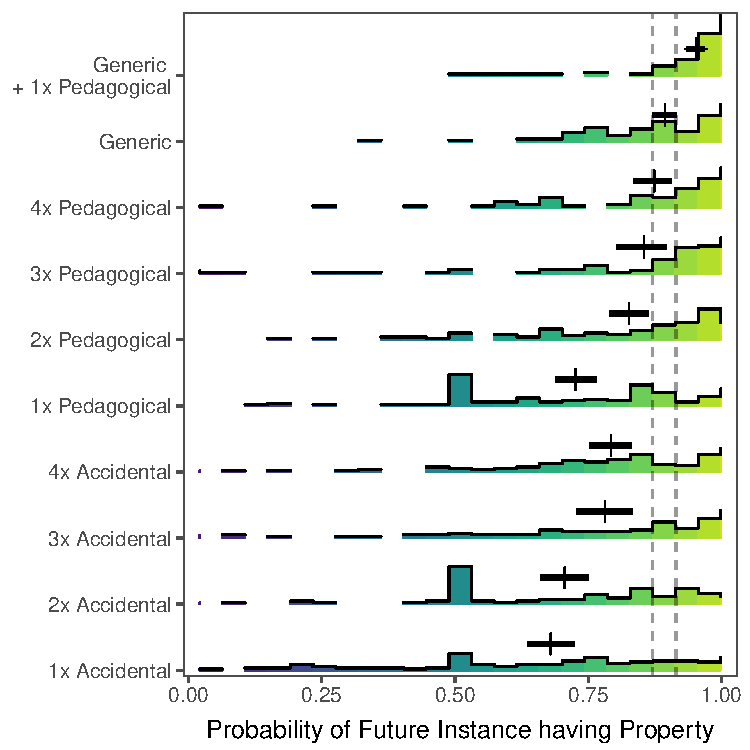
\includegraphics[width=\linewidth]{figs/genex-pilots_10conditions_reordered.pdf}
\end{center}
\caption{Experiment 1 results. Histograms of  Means and 95\% bootstrapped confidence intervals appear above the empirical histograms. Dotted lines represented the confidence interval for the generic only condition. Visually, it appears that the generic is worth about 2 or 3 pedagogical examples.}
\label{fig:results}
\end{figure}


%To determine how many observations one generic is worth
%
%We approach the question of how many observations one generic is worth from a Bayesian modeling perspective. 
%We formalize this question by asking when the distribution of responses for a given experimental condition is more likely to come from the same distribution of responses as the generic condition than it is from a different distribution. That is, we are looking for evidence in support of the null hypothesis that the distribution of responses for one condition is the same as the distribution for another condition. 



\begin{center}
  \begin{table}[h]
    \centering
    \pgfplotstabletypeset[sci zerofill,
    col sep = comma,
    every head row/.style={before row = \toprule, after row = \midrule},
    every last row/.style={after row = \bottomrule},
    columns/condition/.style={string type, column name={Comparison}, column type = l},
    columns/bf/.style={column name={Bayes Factor}, dec sep align},
    columns/logbf/.style={column name={log BF}, sci sep align}]
    {output_from_r/n_obs_bf_5000k_5000k.csv}
    \caption{Experiment 1 model comparison. Bayes Factors in support of the hypothesis that the strength of generalization implied by a generic is equal to that of the experimental condition.}
    \label{tab:nobsBF}
  \end{table}
\end{center}

%\subsubsection{Results}
The question of how many observations one generic is worth is a natural question from a Bayesian hypothesis testing framework, where one can quantify the amount of evidence in support of a null hypothesis that two distributions are in fact the same (i.e., evidence in support of no-difference between conditions).

\noindent\textbf{Linking function}
In order to faithfully model the distribution of responses in each of the experimental conditions, we first perform a Bayesian analysis to determine the best function that characterizes our response variable, since they are clearly not normally distributed.
Since the slider bar ratings we acquire are values between 0 and 1, we assume the distribution of responses is a mixture of some number of Beta distributions (which have support defined over 0 and 1).\footnote{The Beta distribution is defined over the open interval (0, 1), whereas our response variable could contain the endpoints 0 and 1. To accommodate responses that are exactly 0 or exactly 1, we adjust these end-point responses to be equal to 0.001 and 0.999, respectively.}

We model the data for each condition independently with either a single Beta distribution, a mixture of two Betas, or a mixture of three Betas.
We parameterize the Beta components using their mean $\mu$ and concentration $\xi$ parameterization, and put the following priors over the parameters: $\mu_i \sim \text{Uniform}(0,1)$ and $\xi_i \sim \text{Exponential}(1)$. 
The priors on mixture components $\phi$ followed uninformative Dirichlet priors: $\phi \sim \text{Dirichlet}(1, 1, 1)$.
To compute the marginal likelihoods of the data for each model, we used an Annealed Importance Sampling algorithm \cite{neal2001annealed} implemented in the probabilistic programming language WebPPL \cite{dippl}. 

We compute Bayes Factors by comparing the marginal likelihood of the data under each hypothesis about the number of mixture components ($N = \{1, 2, 3\}$).
We find that the data is much more likely to come from a mixture of Beta distributions than a single distribution (BF $\approx 10^{20}$), though the data is inconclusive as to whether or not it is a mixture of two distributions or of three (BF = 0.64). %Table~\ref{tab:componentBF}). 
Since the data is inclusive between two- and three- mixture components, we use a mixture of two distributions to characterize the responses for computational simplicity. 

\noindent\textbf{Bayesian analysis}
Having determined the best linking function for the distribution of responses, we perform a Bayesian analysis to determine which---if any---of the results of our experimental conditions is equivalent to the results of the Generic Only condition. 
We do this by computing the marginal likelihood of the combined data set of the Generic condition and one of the other experimental conditions under the assumption that they are generated from the same distribution (i.e., the same two-component mixture-of-Betas model). 
We compare this likelihood to that calculated by assuming the two conditions were generated by independent distributions (i.e, two different two-component mixture-of-Beta distributions). 
The comparison of these marginal likelihoods gives us the Bayes Factor quantifying the evidence in support of the hypothesis that two conditions were generated from the same underlying distribution (i.e., the generic is worth $n$ observations). 
The results are shown in Table \ref{tab:nobsBF}.

Foremost, there is strong evidence against the hypothesis that a generic is worth a single positive observation, even one presented pedagogically.
The evidence is the strongest that 4 pedagogical examples is worth the same as a generic, but already at 2 pedagogical examples we do see strong evidence for the equivalence. 
Interestingly, at no point are the accidental examples equal to the generic.








\begin{figure}[t]
\begin{center}
 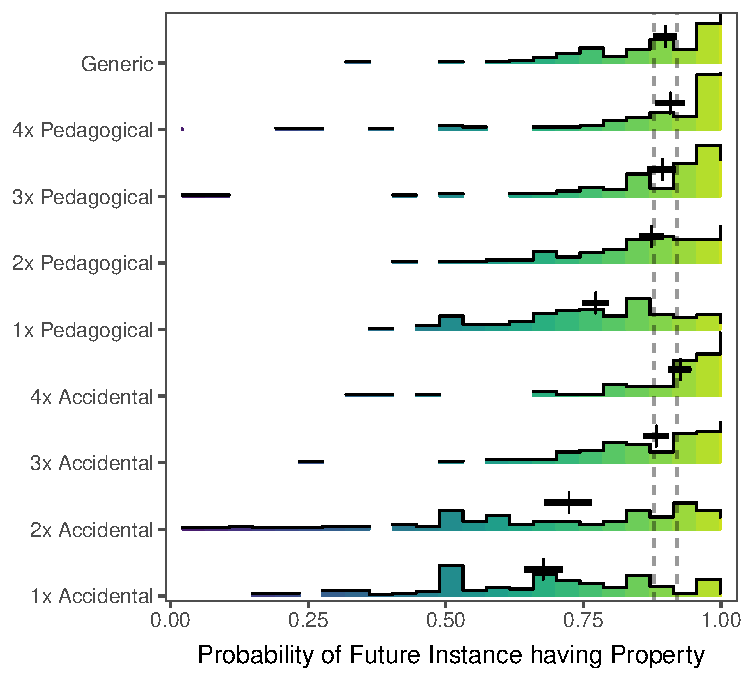
\includegraphics[width=\linewidth]{figs/genex-expt2_9conditions_reordered.pdf}
\end{center}
\caption{Experiment 2 results when feature is articulated explicitly. Means and 95\% bootstrapped confidence intervals appear above the empirical histograms. Dotted lines represented the confidence interval for the Generic Only condition (Experiment~1). Data for the generic condition is copied from Experiment~1 (top row).}
\label{fig:results2}
\end{figure}
\subsection{Experiment 2}

In Experiment 1, we compared the inductive strength of learning from a generic sentence (e.g., ``Feps have white wings'') to learning from pedagogically or accidentally demonstrated examples (e.g., observing a fep with a white wing). 
One difficulty in learning from examples is that an individual instance of a category appears with many features presented simultaneously. 
Thus, one way in which generic language can foster generalization is by individuating the feature to be generalized. In Experiment 1, the feature being demonstrated was never named (i.e., the demonstrator just said ``Look at this" and a feature was either pointed out or in the accidental case, not indicated directly at all), leaving ambiguity about the exact feature being pedagogically highlighted or accidentally observed. In the Generic Only and Generic + Pedagogical Example condition, however, the feature of interest was identified linguistically, eliminating such ambiguity (e.g., ``Feps have white wings.").
To control for the possibility that individuating a feature is what enabled stronger generalizations from a generic than from a single observation in Experiment~1, we ran a follow-up experiment in which the learning events involving observations also included the labeling of the property. \soph{Tried to be a bit more explicit about what was going on in the experiment and the possibility we are controlling for. Please double check to make sure I haven't misconstrued anything.}

\subsubsection{Participants and procedure}

We collected data from 378 participants recruited from Amazon Mechanical Turk.
For this experiment, we modified the Example conditions from Experiment 1, so participants were either assigned to the Pedagogical Example or Accidental Example condition and observed 1, 2, 3, or 4 exemplars (i.e., 8 conditions total). The Example conditions were modified such that the scientist provided both the label for the category and the name of the feature. In the Pedagogical Example, after naming the category (e.g., ``This is a...''/ ``These are 2/3/4...''), he said, ``I have something to show you'' and then named the feature as the bird or flower enlarged (``White Wings/A black center'') or as the artifact dropped and squeaked "Squeaking".
In the Accidental Example, as the bird or flower enlarged, the scientist said, ``Oh, Look at that! White wings/A black center'' and when the artifact dropped and squeaked, he said, ``Oops! Listen to that! Squeaking!'' 

\subsubsection{Results}

Figure \ref{fig:results2} shows the responses for each condition in this experiment, with the data from the Generics Only condition of Experiment~1 reproduced for easier comparison. 
As in Experiment~1, we see that the change in distributions with increasing examples in the Pedagogical~vs.~Accidental Example conditions is different. We observe a bi-modality in the distribution of responses in both the pedagogical and accidental conditions, and again the bi-modality disappears after 3 observations for the Accidental condition and after 2 observations for the Pedagogical condition. We see some evidence as well that labeling the feature strengthens generalizations from examples (compared to Experiment~1 where the features were not labeled), a point we return to in the discussion.

\section{Discussion}

Successfully navigating the environment requires anticipating what is to come, and abstract generalizations allow us to reason flexibly about instances of categories and events that we have not yet experienced. 
These generalizations can be constructed both by directly observing instances in the world and by being told the generalization in the form of a generic sentence. 
But what is the relationship between learning from examples and learning from generics? 
Here we ask a simple question: How many observations is one generic worth?
We find that, contra extant theoretical proposals, the strength of the generalization implied by a generic is equivalent to at least two pedagogically-sampled examples. 

In our second experiment, we saw suggestive evidence that describing the feature explicitly (e.g., ``white wings'') led to stronger generalizations than not describing the features with language. 
This points to an interesting dissection of the content of the generalization implied by generics. Part of the content of the generalization comes from simply articulating the feature. This implication of the label makes sense.  Generics are one of the most primitive syntactic and semantic constructions: nearly anytime you put a category and a property label together, you can get a generic meaning (e.g., ``A dog barks''). 
%In our experiment, we used predicates that are directly observable---sounds that an animal or object could make---and that could plausibly be construed as idiosyncratic properties of individuals (e.g., \emph{This fep squawks}) or characteristic properties of categories (e.g., it is typical of feps to squawk).
%Observing different kinds of properties in general should lead to different strengths of generalization implied by examples \cite{Nisbett1983}. 
%Does this imply that the examples---generics exchange rate is different for generalizing different properties?
%Not necessarily.
%It is also the case that the strength of generalization implied by a generic varies by the type of property \cite{Tessler2020}. 
%In fact, it is a prediction of the theory of \citeA{Tessler2019, Tessler2020} that the exchange rate will be the same across properties. (What is different across properties, according to \cite{tessler2019language}, is the prior knowledge.)

In our experiment, we also used novel categories that would plausibly be construed as subordinate level categories (i.e., a fep is a type of bird).
We focus on subordinate level categories to isolate the contribution of the number of examples without concern as to the differences or variability among the examples with respect to the extension of the category.
That is, the generics--examples exchange-rate will, in general, depend upon the level of abstraction of the category. 
Learning from examples the same kind of generalization as that conveyed with a generic about a superordinate category (e.g., ``Mammals are warm-blooded'') will be much more difficult than the subordinate categories we used. 
In particular, to make a strong generalization to the category of mammals, a learner would benefit from a diverse set of examples (e.g., bears, cats, whales, ...) and in addition significantly benefit from prior knowledge that different animal families have a consistent kind of bloodedness. 
The power of generics then scales with the level of abstraction of the category: Generics about more abstract, superordinate categories will, in general, be harder to learn from examples than generics about basic level or subordinate level categories. 

%\subsection{Relationship to children}

%\mht{Changes from infancy to early childhood?}

%\mht{Changes across childhood?}

%\subsection{Relation to other tasks}

Our experimental method is similar but distinct from other studies investigating the interpretation of generics vis a vis examples or statistics.
\citeA{Cimpian2010a} compared the strength of generalization implied by a generic (what they called \emph{implied prevalence}) to the statistics of the feature in terms of its prevalence in the category that led participants to endorse the generic (what they call \emph{truth conditions}). \soph{Can you be more specific here/give a concrete example of the stimuli? It's not clear what the statistics of the feature in terms of its prevalence in the category means or how it translates to an empirical method...as you do for Kushnir below}They found that generics (at least, generics about the kinds of predicates they tested) tend to be interpreted more strongly than what one would expect given the statistical information that lead people to endorse generics. 

\citeA{kushnir2016translating} examined the strength of generalizations and trust in informants after jointly hearing generic language and observing some number of instances of the category with/without the property (e.g., hearing ``Blickets squeak'' and then observing 2 out of 10 blickets squeak).
This paradigm is an indirect measure of the generics--examples exchange-rate because it incorporates the additional variable of trust in testimony.
That is, a learner can explain away conflicting observations and testimony through two means: (a) weakening the generalization strength implied by the generic (e.g., \emph{the speaker did not mean most exemplars have the property but rather only some}) and (b) weakening trust in the speaker (e.g., \emph{the speaker was ill-informed}). 
This interplay between the vagueness of generics and speaker trust is a complex problem that should receive more attention in its own right. \soph{In a sense we also look at speaker trust but in terms of the manner of the demonstration (accidental vs. generic); i.e., we manipulate plausible knowledge by the means of demosntration rather than negative examples. my attempt is below but I think it is too long}

Our paradigm touches on the idea of speaker trust or implied speaker knowledge by manipulating the intentionality of the demonstration. While \citeA{kushnir2016translating} find that the number of positive or negative examples can increase or undermine trust in a speaker's testimony, we find that pedagogical vs. accidental demonstration informs the strength of the generalization adults draw from one or multiple examples. Such strengthening is consistent with children's interpretation of intentional vs. accidental actions in terms of which actions they should imitate and how broadly or persistently they should explore~\cite<e.g.,>{bonawitz2011double, butler2012preschoolers}. 

%\subsection{Other limitations of this study}

One limitation of our paradigm that we wish to highlight is that our paradigm does not evoke uninhibited, automatic, bonafide communicative reasoning but rather is embedded in a story book that depicts certain communicative acts %\red{(cite Clark?)}. 
For example, the Accidental Example condition is not really incidental: We designed the task in order to depict an accident, and our participants are presumably aware of this. 
We find that participants interpret the evidence presented in the Accidental Example conditions in some way weaker than the same evidence presented in the Pedagogical Example conditions, which provides evidence that participants represent these as different events and perhaps recognize our intention to display different events. Thus, what we are tapping into is plausibly not the generalization implied by an incidental observation but rather the generalization that participants believe that others (e.g., the experimenter, the community) might draw from incidental observations. 
We are currently working on an interactive paradigm where participants learn about the world through self-directed, not experimentally supplied, learning events. 

\soph{We need a grand conclusion ;)}


\section{Acknowledgments}


The authors would like to thank Karen Guo for her integral contributions to programming the experiment and data collection. 
This material is based upon work supported by the National Science Foundation SBE Postdoctoral Research Fellowship Grant No.~1911790 awarded to M.H.T., a National Science Foundation Graduate Research Fellowship Grant No.~XXX awarded to S.B., and Army Research Office MURI Grant No. W911NF-19-1-0057.

\bibliographystyle{apacite}

\setlength{\bibleftmargin}{.125in}
\setlength{\bibindent}{-\bibleftmargin}

\bibliography{genex_cogsci20}


\end{document}
